% Chapter 2
\chapter{Digital Signal Process} % Main chapter title

\label{Chapter2} % For referencing the chapter elsewhere, use \ref{Chapter1}

\lhead{Chapter 2. \emph{Digital Signal Process}} % This is for the header on each page - perhaps a shortened title

\cite{wiki-dsp-sampling}
Sampling is the process of recording the values of a signal at given points in time. For A/D converters, these points in time are equidistant. The number of samples taken during one second is called the sample rate. Keep in mind that these samples are still analogue values. The mathematic description of the ideal sampling is the multiplication of the signal with a sequence of dirac pulses. In real A/D converters the sampling is carried out by a sample-and-hold buffer. The sample-and-hold buffer splits the sample period in a sample time and a hold time. In case of a voltage being sampled, a capacitor is switched to the input line during the sample time. During the hold time it is detached from the line and keeps its voltage.

\begin{figure}[ht]
  \centering
    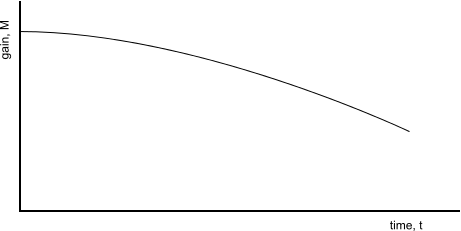
\includegraphics[width=0.7\textwidth, keepaspectratio=true]{chap2-Analog_Waveform.png}
  \caption{}
  \label{fig:chap2-Analog_Waveform}
\end{figure}

\begin{figure}[ht]
  \centering
    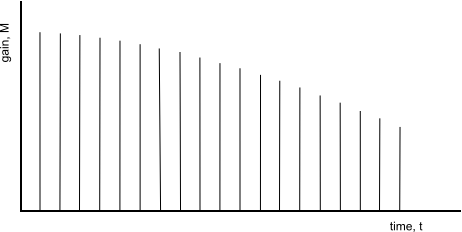
\includegraphics[width=0.7\textwidth, keepaspectratio=true]{chap2-Sampled_Waveform.png}
  \caption{}
  \label{fig:chap2-Sampled_Waveform}
\end{figure}

\section{ADC and DAC}\cite{smith1997dspbook}
Most of the signals directly encountered in science and engineering are continuous: light intensity that changes with distance; voltage that varies over time; etc. Analog-to-Digital Conversion (ADC) and Digital-to-Analog Conversion (DAC) are the processes that allow digital computers to interact with these everyday signals. Digital information is different from its continuous counterpart in two important respects: it is sampled, and it is quantized. Both of these restrict how much information a digital signal can
contain. This chapter describes the sampling frequency, number of bits, and type of analog filtering needed for converting between the analog and digital.

\begin{compactitem}
\item \textbf{Quantization}
Quantization is the process of representing the analog voltage from the sample-and-hold circuit by a fixed number of bits. The input analog voltage (or current) is compared to a set of pre-defined voltage (or current) levels. Each of the levels is represented by a unique binary number, and the binary number that corresponds to the level that is closest to the analog voltage is chosen to represent that sample. This process rounds the analog voltage to the nearest level, which means that the digital representation is an approximation to the analog voltage. There are a few methods for quantizing samples. The most commonly used ones are the dual slope method and the successive approximation.

\begin{figure}[ht]
  \centering
    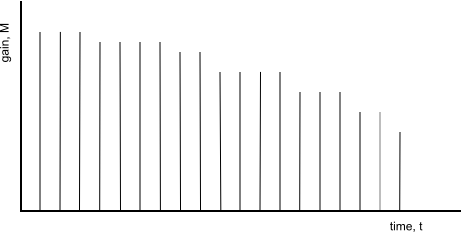
\includegraphics[width=0.7\textwidth, keepaspectratio=true]{chap2-Digital_Waveform.png}
  \caption{}
  \label{fig:chap2-Digital_Waveform}
\end{figure}


\item \textbf{The Sampling Theorem}\cite{dsp-nyquist}\\
The sampling theorem states that for a limited bandwidth (band-limited) signal with maximum frequency $f_{max}$, the equally spaced sampling frequency $f_s$ must be greater than twice of the maximum frequency $f_{max}$, i.e.,
$f_s > 2·f_{max}$
in order to have the signal be uniquely reconstructed without aliasing.

The frequency $2·f_{max}$ is called the \textbf{Nyquist sampling rate}. Half of this value, $f_{max}$, is sometimes called the \textbf{Nyquist frequency}.

\end{compactitem}

\section{Fourier Transform} \cite{csulb-Woollett}

\begin{compactitem}

\item {Fourier Series Expansion of a Function over $(-\boldsymbol{\pi,\,\pi})$}\\
A Fourier series expansion designed to represent a given function
  \textbf{f(x)} defined over a finite interval $(-\boldsymbol{\pi, \pi})$, is a sum of terms
\begin{equation}  \label{fxpi}
\mathbf{f(x) = \frac{1}{2} \, a_{0} + \sum_{n=1}^{\infty} \left[
   a_{n}\,\boldsymbol{\cos} (n\,x) + b_{n} \,\boldsymbol{\sin} (n\,x) \right] }
\end{equation}

\noindent and the constant coefficients ($\mathbf{a_{n},\, b_{n}}$) are
\begin{equation} \label{fcoeff}
 \mathbf{ a_{n} = \frac{1}{\boldsymbol{\pi}} \, \int_{-\boldsymbol{\pi}}^{\boldsymbol{\pi}} f(y)\,
   \boldsymbol{\cos} (n\,y) \, dy}, \quad
   \mathbf{ b_{n} = \frac{1}{\boldsymbol{\pi}} \, \int_{-\boldsymbol{\pi}}^{\boldsymbol{\pi}} f(y)\,
   \boldsymbol{\sin} (n\,y) \, dy}.
\end{equation}
(For a derivation of these equations see Sec.\ref{expfs} and Eqs.(\ref{Eq:piex1}) and
  (\ref{Eq:piex2}).)\\

\noindent The first term of the expansion
\begin{equation}
\mathbf{ \frac{1}{2} \, a_0  =
 \frac{1}{2\, \boldsymbol{\pi}}  \int_{-\boldsymbol{\pi}}^{\boldsymbol{\pi}} f(y)\,dy =
 \langle f(x) \rangle }
\end{equation}
is the (un-weighted) average of \textbf{f(x)} over the domain $(-\boldsymbol{\pi},\boldsymbol{\pi})$.
Hence $\mathbf{a_{0}}$ will always be twice the average value of the function over
  the domain.\\

\noindent If \textbf{f(x)} is an even function ($\mathbf{f(-x) =  f(x)}$),
  then only the $\mathbf{\boldsymbol{\cos}(n\,x)}$ terms
  contribute.
If \textbf{f(x)} is an odd function ($\mathbf{f(-x) =  -f(x)}$),
  then only the $\mathbf{\boldsymbol{\sin}(n\,x)}$ terms contribute. \\


\item {Fourier Transform}\\
\textbf{Fourier Cosine Integrals}
Given some function $\mathbf{f(x)}$ defined for $\mathbf{x \geq 0}$,
  we define the Fourier cosine transform  of this function as
\begin{equation}  \label{Eq:fc1}
\mathbf{F_{C}(f,\boldsymbol{\omega}) = \frac{2}{\boldsymbol{\pi}}
  \int_{0}^{\infty} \boldsymbol{\cos}(\boldsymbol{\omega}\,x)\,f(x)\,dx }
\end{equation}
The given function $\mathbf{f(x)}$ can then be written as an integral
  over positive values of $\boldsymbol{\omega}$:
\begin{equation}  \label{Eq:fc2}
\mathbf{f(x) = \int_{0}^{\infty} F_{C}(f,\boldsymbol{\omega})\,
    \cos(\boldsymbol{\omega}\,x)\,d\boldsymbol{\omega} }
\end{equation}
The two equations (\ref{Eq:fc1}) and (\ref{Eq:fc2}) are an example of
  a "Fourier transform pair", which include conventions about where
  to place the factor of $2/\boldsymbol{\pi}$.\\

\textbf{Fourier Sine Integrals}\\
Given some function $\mathbf{f(x)}$ defined for $\mathbf{x \geq 0}$,
  we define the Fourier sine transform  of this function as
\begin{equation}  \label{Eq:fsine1}
\mathbf{F_{S}(f,\boldsymbol{\omega}) = \frac{2}{\boldsymbol{\pi}}
  \int_{0}^{\infty} \boldsymbol{\sin}(\boldsymbol{\omega}\,x)\,f(x)\,dx }
\end{equation}
The given function $\mathbf{f(x)}$ can then be written as an integral
  over positive values of $\boldsymbol{\omega}$:
\begin{equation}  \label{Eq:fsine2}
\mathbf{f(x) = \int_{0}^{\infty} F_{S}(f,\boldsymbol{\omega})\,
    \sin(\boldsymbol{\omega}\,x)\,d\boldsymbol{\omega} }
\end{equation}
The two equations (\ref{Eq:fsine1}) and (\ref{Eq:fsine2}) are another
   "Fourier transform pair", which include conventions about where
  to place the factor of $2/\boldsymbol{\pi}$.

\textbf{Exponential Fourier Integrals}\\
Given some function $\mathbf{f(x)}$ defined for $\mathbf{-\infty <x < \infty}$,
  we define the exponential Fourier transform  of this function as
\begin{equation}  \label{Eq:fexp1}
\mathbf{F_{Exp}(f,\boldsymbol{\omega}) = \frac{1}{2\, \boldsymbol{\pi}}
  \int_{-\infty}^{\infty} \,f(x) e^{i\,\boldsymbol{\omega}\,x}\,dx }
\end{equation}
The given function $\mathbf{f(x)}$ can then be written as an integral
  over both positive and negative values of $\boldsymbol{\omega}$:
\begin{equation}  \label{Eq:fexp2}
\mathbf{f(x) = \int_{-\infty}^{\infty} F_{Exp}(f,\boldsymbol{\omega})\,
    e^{-i\,\boldsymbol{\omega}\,x} \,d\boldsymbol{\omega} }
\end{equation}
The two equations (\ref{Eq:fexp1}) and (\ref{Eq:fexp2}) are another
   "Fourier transform pair", which include conventions about where
  to place the factor of $\mathbf{2\, \boldsymbol{\pi}}$ as well as which member
  has the minus sign in the exponent.\\

\noindent If the given function is even, $\mathbf{f(-x) = f(x) }$, then the
exponential Fourier transform has the symmetry
\begin{equation}
\mathbf{F_{Exp}(f,\boldsymbol{-\omega}) = F_{Exp}(f,\boldsymbol{\omega}) }
\end{equation}
and can be expressed in terms of the Fourier cosine transform:
\begin{equation}
\mathbf{F_{Exp}(f,\boldsymbol{\omega}) = \frac{1}{2} \, F_{C}(f,\boldsymbol{\omega})}.
\end{equation}
If the given function is odd, $\mathbf{f(-x) = -f(x) }$, then the
exponential Fourier transform has the symmetry
\begin{equation}
\mathbf{F_{Exp}(f,\boldsymbol{-\omega}) = -F_{Exp}(f,\boldsymbol{\omega}) }
\end{equation}
and can be expressed in terms of the Fourier sine transform:
\begin{equation}
\mathbf{F_{Exp}(f,\boldsymbol{\omega}) = \frac{i}{2} \, F_{S}(f,\boldsymbol{\omega})}.
\end{equation}
If the given function is neither even nor odd, the function can always be written
  as the sum of an even function $\mathbf{f_{e}(x)}$ and an odd function $\mathbf{f_{o}(x)}$:
\begin{equation}
\mathbf{f(x) \equiv f_{e}(x) + f_{o}(x) =
  \frac{1}{2} \,( f(x) + f(-x) + \frac{1}{2} \, ( f(x) - f(-x) }
\end{equation}
and can be expressed in terms of the Fourier cosine transform of $\mathbf{f_{e}(x)}$
  and the Fourier sine transform of $\mathbf{f_{o}(x)}$:
\begin{equation}
\mathbf{F_{Exp}(f,\boldsymbol{\omega}) \equiv F_{Exp}(f_{e}+f_{o},\boldsymbol{\omega}) =
  \frac{1}{2} \, F_{C}(f_{e},\boldsymbol{\omega}) +
  \frac{i}{2} \, F_{S}(f_{o},\boldsymbol{\omega}) }
\end{equation}


\item {Discrete Fourier Transform}

\item {Fast Fourier Transform}

\item {Power Spectra}

\end{compactitem}

%----------------------------------------------------------------------------------------

\section{ICA}
Independent Component Analysis (ICA) is a computationally efficient blind source separation technique.
It has been an area of interest for researchers for many practical applications in various fields of science and
engineering.

\cite{journals/informaticaSI/NaikK11}
\begin{compactitem}

\item {Introduction}
The problem of source separation is an inductive inference problem. There is not enough information
to deduce the solution, so one must use any available information to infer the most probable solution.
The problem of separating and estimating the original source waveforms from the sensor array, 
without knowing the transmission channel characteristics and the source can be briefly expressed
as problems related to BSS. In BSS the word blind refers to the fact that we do not know how the signals
were mixed or how they were generated. As such, the separation is in principle impossible. Allowing some relatively indirect and general constrains, we however still hold the term BSS valid, and separate under these conditions. There appears to be something magical about blind source separation; we are estimating the original source signals without knowing the parameters of mixing and/orfiltering processes. Independent component analysis (ICA) is one of the most widely used BSS techniques for revealing hidden factors that underlie sets of random variables, measurements, or signals. ICA is essentially a method for extracting individual
signals from mixtures. Its power resides in the physical assumptions that the different physical processes
generate unrelated signals. The simple and generic nature of this assumption allows ICA to be successfully applied in diverse range of research fields. The BSS is unsupervised and thought of as a black box method.

\item {ICA model}
The general model for ICA is that the sources are generated
through a linear basis transformation, where additive
noise can be present. Suppose we have N statistically independent
signals, si(t), i = 1, ...,N. We assume that the
sources themselves cannot be directly observed and that
each signal, si(t), is a realization of some fixed probability
distribution at each time point t. Also, suppose we observe
these signals using N sensors, then we obtain a set of N observation
signals xi(t), i = 1, ...,N that are mixtures of the
sources. A fundamental aspect of the mixing process is that
the sensors must be spatially separated (e.g. microphones
that are spatially distributed around a room) so that each
sensor records a different mixture of the sources. With this
spatial separation assumption in mind, we can model the
mixing process with matrix multiplication as follows:

\begin{equation}
\label{eq:ica-linear}
\\
x(t) = As(t)
\end{equation}\\

where A is an unknown matrix called the mixing matrix
and $x(t), s(t)$ are the two vectors representing the observed
signals and source signals respectively. Incidentally, the
justification for the description of this signal processing
technique as blind is that we have no information on the
mixing matrix, or even on the sources themselves.
The objective is to recover the original signals, $s_i(t)$,
from only the observed vector $x_i(t)$. We obtain estimates
for the sources by first obtaining the “unmixing matrix” $W$,
where, 
This enables an estimate, $\hat{s}(t)$, of the independent
sources to be obtained:

\begin{equation}
\label{eq:ica-white}
\hat{s}(t) =Wx(t)
\end{equation}\\

The diagram in Figure 1 illustrates both the mixing
and unmixing process involved in BSS. The independent
sources are mixed by the matrix A (which is unknown in
this case). We seek to obtain a vector y that approximates
s by estimating the unmixing matrix W. If the estimate of
the unmixing matrix is accurate, we obtain a good approximation
of the sources.
The above described ICA model is the simple model
since it ignores all noise components and any time delay
in the recordings.
\item {Independence}

A key concept that constitutes the foundation of independent
component analysis is statistical independence. To
simplify the above discussion consider the case of two different
random variables s1 and s2. The random variable s1
is independent of s2, if the information about the value of
s1 does not provide any information about the value of s2,
and vice versa. Here s1 and s2 could be random signals
originating from two different physical process that are not
related to each other.

\begin{figure}[ht]
  \centering
    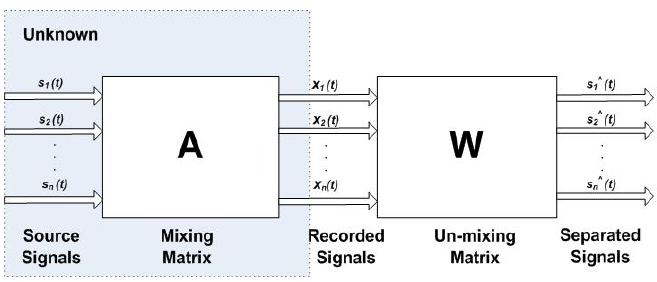
\includegraphics[width=0.7\textwidth, keepaspectratio=true]{chap2-ICA.png}
  \caption{Blind source separation (BSS) block diagram. $s(t)$ are the sources. $x(t)$ are the recordings,
	$\hat{s}(t)$ are the estimated sources A is mixing matrix and W is un-mixing matrix. }
  \label{fig:chap2-ICA}
\end{figure}

\item {Preprocessing}
Before examining specific ICA algorithms, it is instructive
to discuss preprocessing steps that are generally carried out
before ICA.

\item {Centering}
A simple preprocessing step that is commonly performed
is to “center” the observation vector x by subtracting its
mean vector $m=E{x}$. That is then we obtain the centered
observation vector, $x_c$, as follows:
\begin{equation}
\label{eq:ica-zero-mean}
x_c = x-m
\end{equation}

This step simplifies ICA algorithms by allowing us to
assume a zero mean. Once the unmixing matrix has been
estimated using the centered data, we can obtain the actual
estimates of the independent components as follows:

\begin{equation}
\label{eq:ica-source}
\hat{s}(t) = A^{-1} (x_c + m )
\end{equation}

From this point on, all observation vectors will be assumed
centered. The mixing matrix, on the other hand,
remains the same after this preprocessing, so we can always
do this without affecting the estimation of the mixing
matrix.

\item {Whitening}
Another step which is very useful in practice is to prewhiten
the observation vector x. Whitening involves linearly
transforming the observation vector such that its components
are uncorrelated and have unit variance . Let
xw denote the whitened vector, then it satisfies the following
equation:
\begin{equation}
\label{eq:ica-source1}
E{x_w x^T_w} = I
\end{equation}

where $E{x_w x^T_w}$ is the covariance matrix of $x_w$. Also,
since the ICA framework is insensitive to the variances
of the independent components, we can assume without
loss of generality that the source vector, s, is white, i.e.
$E{s s^T } = I$
A simple method to perform the whitening transformation
is to use the eigenvalue decomposition (EVD) of x. 
That is, we decompose the covariance matrix of x as follows:
\begin{equation}
\label{eq:ica-evd}
E{x x^T } =VDV^T
\end{equation}
where V is the matrix of eigenvectors of $E{x x^T }$,
and D is the diagonal matrix of eigenvalues, i.e. 
$D = diag{\lambda_1,\lambda_2, ...,\lambda_n}$. The observation vector can be
whitened by the following transformation:
\begin{equation}
\label{eq:ica-whiteningX1}
x_w = VD^{-1/2}V^Tx
\end{equation}
where the matrix $D^{-1/2}$ is obtained by a
simple component wise operation as $D^{-1/2}=diag{\lambda_1^{-1/2},\lambda_2^{-1/2},...,\lambda_n^{-1/2}}$. Whitening transforms
the mixing matrix into a new one, which is orthogonal
\begin{equation}
\label{eq:ica-whiteningX}
x_w=VD^(-1/2)V^TAs=A_w s
\end{equation}

hence,
\begin{equation}
\label{eq:ica-CoVI}
E{x_w x^T_w } = A_w E{s s^T }A^T_w
= A_w A^T_w = I
\end{equation}

Whitening thus reduces the number of parameters to be
estimated. Instead of having to estimate the $n^2$ elements of
the original matrix A, we only need to estimate the new orthogonal
mixing matrix, where An orthogonal matrix has
$n(n-1)/2$ degrees of freedom. One can say that whitening
solves half of the ICA problem. This is a very useful step
as whitening is a simple and efficient process that significantly
reduces the computational complexity of ICA. An illustration
of the whitening process with simple ICA source
separation process is explained in the later section.

\item {ICA Algorithms}
There are several ICA algorithms available in literature.
However the following algorithms are widely used
in numerous signal processing applications. These includes
FastICA, JADE, and ICA RADICAL. Each algorithm used a different
approach to solve equation. We will use ICA RADICAL \cite{radical-ica} to solve our PPG problem.

\end{compactitem}

